% !TeX spellcheck = en_US
\chapter{Evaluation}\label{ch:evaluation}

This chapter is about the evaluation of the several approaches presented in Ch.~\ref{ch:approach}.

\section{Experimental Setup}

For the following evaluations HDT-Java 2.0~\footnote{\label{foot:1}https://github.com/rdfhdt/hdt-java/releases/tag/v2.0} (the currently newest version) has been used. For GRP the implementation mentioned in~\cite{maneth} has been used (written in Scala). It is not open source and has been given to us by the authors of~\cite{maneth}.

\section{HDT vs GRP}\label{sec:evaluationHDTvsGRP}


Fig.~\ref{fig:ratiosHDTWithoutDict} shows the compression ratio for HDT (without dictionary size). As expected, the ratio gets higher the more similar the graph is to the authority pattern. In general it can be said that this effect is quite small. There is only a distance of 0.002 between the minimum and the maximum. This small effect can also be seen by looking at Fig.~\ref{fig:ratiosHDTWithDict}. It can be seen that the size of the dictionary has a much bigger effect, since the compression ratio is now much larger and the curve behavior from Fig.~\ref{fig:ratiosHDTWithoutDict} is no longer recognizable. It is noticeable that the dictionary size gets bigger when the graph is further away from the star pattern. The dictionary implementation of HDT seems to be more inefficient when there are about as many subject as objects. 

\todo{dafür sorgen, dass kurve rechts auch den knick hat}

\begin{figure}[h]
	\centering
	\subfloat[Without dictionary size.]{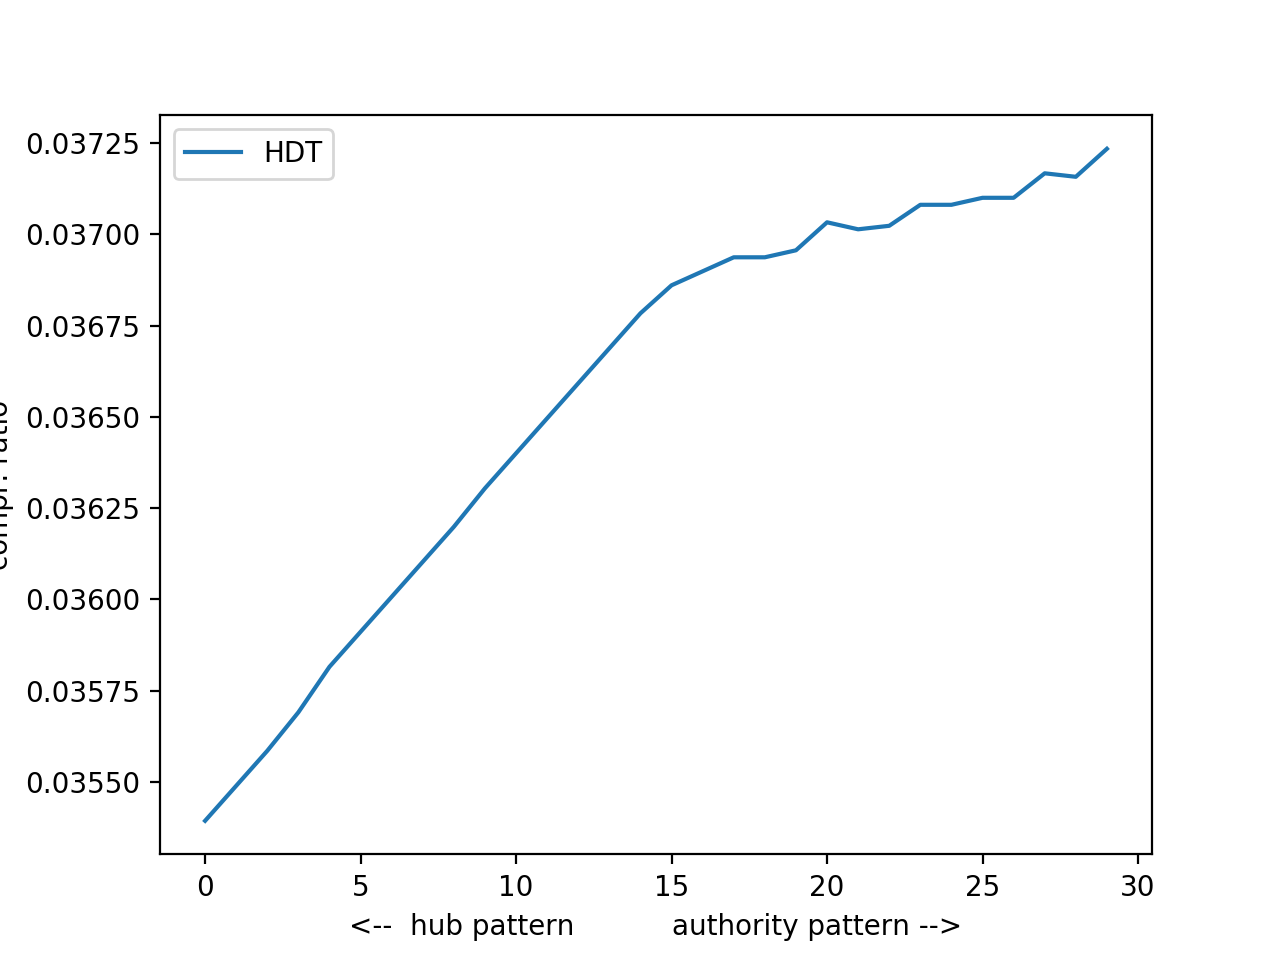
\includegraphics[width=0.5\textwidth]{figures/GRPvsHDT/hdtWithoutDict}\label{fig:ratiosHDTWithoutDict}}
	\hfill
	\subfloat[With dictionary size.]{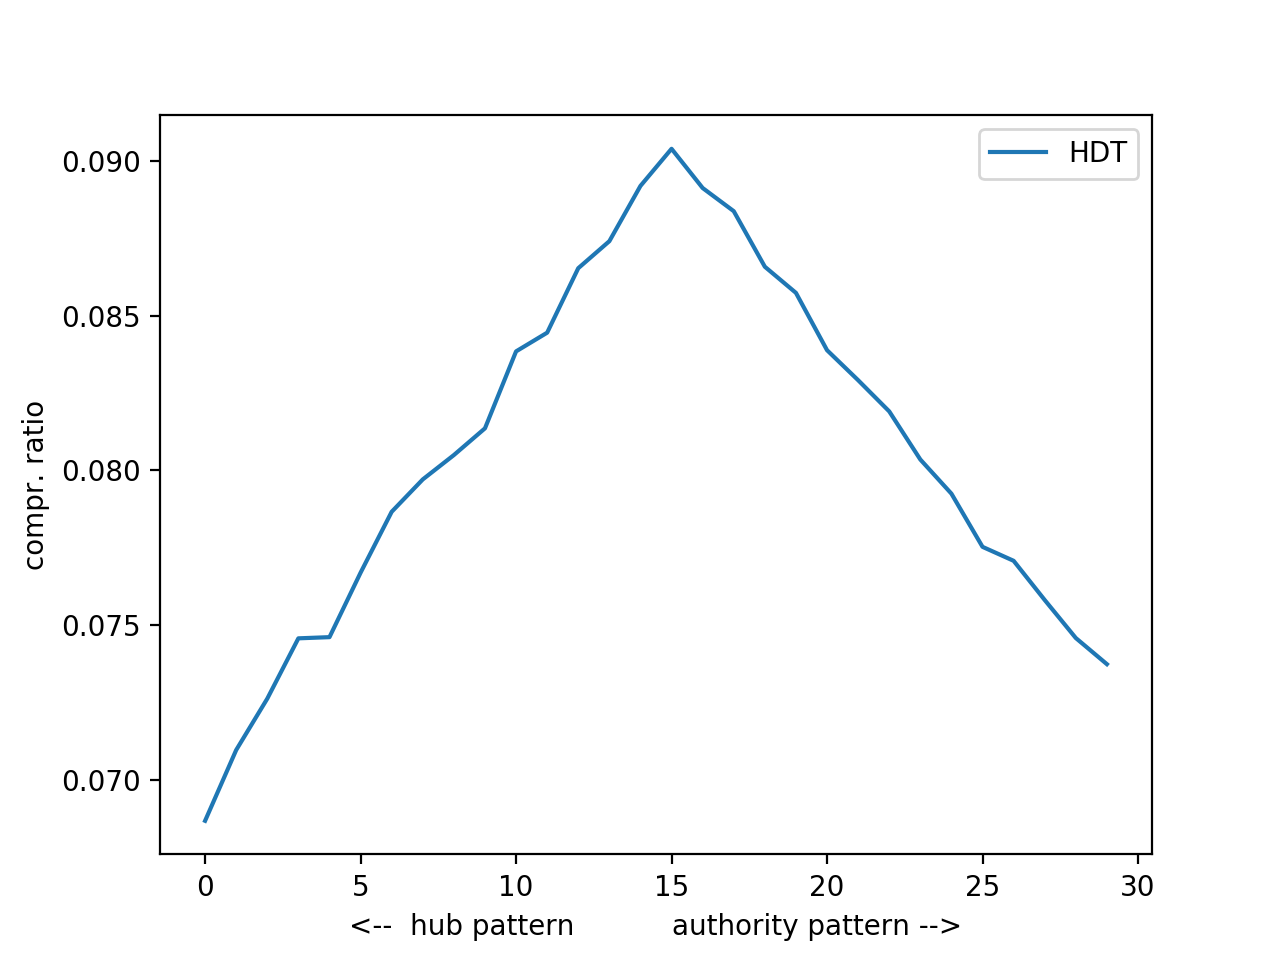
\includegraphics[width=0.5\textwidth]{figures/GRPvsHDT/hdtWithDict}\label{fig:ratiosHDTWithDict}}
	\caption{The compression ratios for HDT without and with dictionary sizes.}
\end{figure}

Next the compression ratio of GRP is considered, which is presented in Fig.~\ref{fig:ratiosGRPWithoutDict} (without dictionary sizes). Here one can see that GRP has a better compression ratio if the graph is more similar to the star pattern (hub order authority pattern). This property of GRP has also been mentioned in~\cite{maneth}. It can also be seen that the effect on the compression ratio is bigger for GRP than for HDT (standard deviation is twice as high for GRP as for HDT). A grammar-based compression is therefore more dependent on the structure of the input data.

When Fig.~\ref{fig:ratiosGRPWithDict} is considered, it can be seen that this curve behaves almost exactly like the one from Fig.~\ref{fig:ratiosHDTWithDict}, since the size of the dictionary accounts for most of the compressed data size.

\begin{figure}[h]
	\centering
	\subfloat[Without dictionary size.]{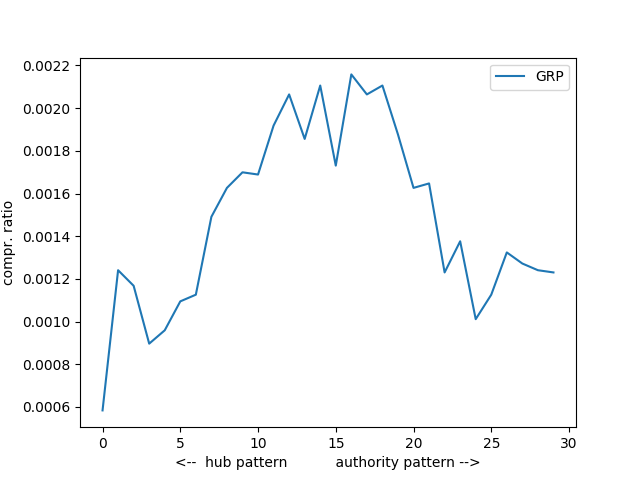
\includegraphics[width=0.5\textwidth]{figures/GRPvsHDT/grpWithoutDict}\label{fig:ratiosGRPWithoutDict}}
	\hfill
	\subfloat[With dictionary size.]{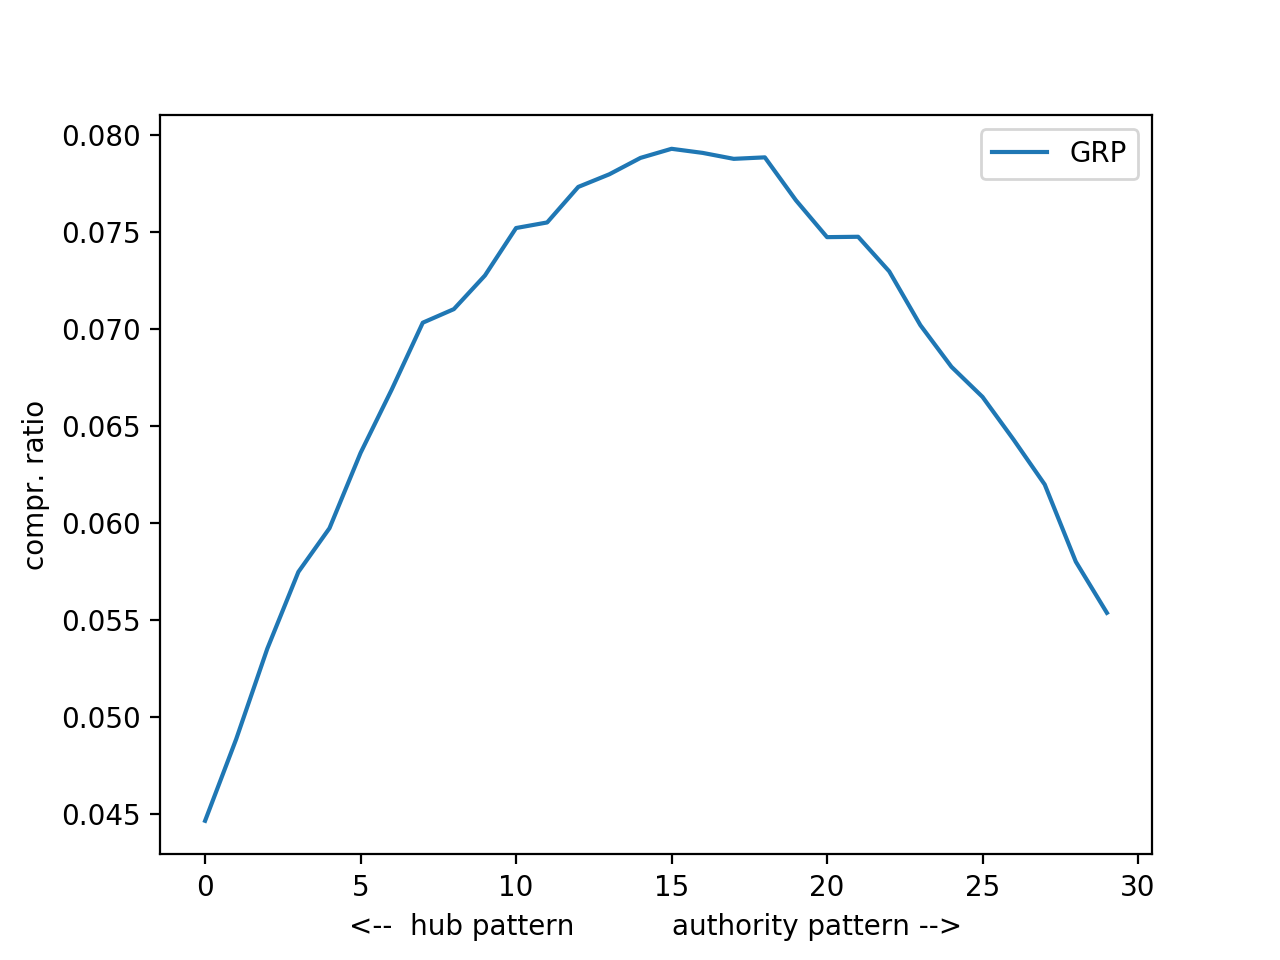
\includegraphics[width=0.5\textwidth]{figures/GRPvsHDT/grpWithDict}\label{fig:ratiosGRPWithDict}}
	\caption{The compression ratios for GRP without and with dictionary sizes.}
\end{figure}

Finally, Fig.~\ref{fig:ratiosBothWithoutDict} and Fig.\ref{fig:ratiosBothWithDict} show the compression ratios for both algorithms. Since both use the same method to compress the dictionary, the curves in Fig.~\ref{fig:ratiosBothWithDict} are very similar. However, it becomes clear that GRP compresses better than HDT. In Fig.~\ref{fig:ratiosBothWithoutDict}, the ratio of HDT is 31 times higher on average. Of course, this factor becomes much smaller in Fig.~\ref{fig:ratiosBothWithDict} because the dictionary accounts for most of the memory size. Here the compression ratio of HDT is on average 1.8 times as high as that of GRP.

\begin{figure}[h]
	\centering
	\subfloat[Without dictionary size.]{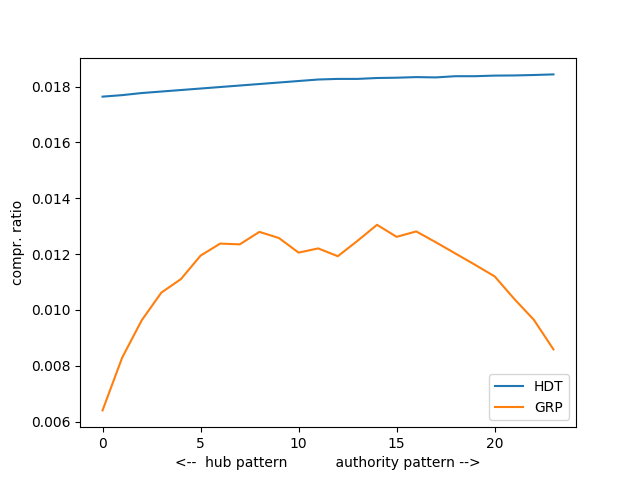
\includegraphics[width=0.5\textwidth]{figures/GRPvsHDT/bothWithoutDict}\label{fig:ratiosBothWithoutDict}}
	\hfill
	\subfloat[With dictionary size.]{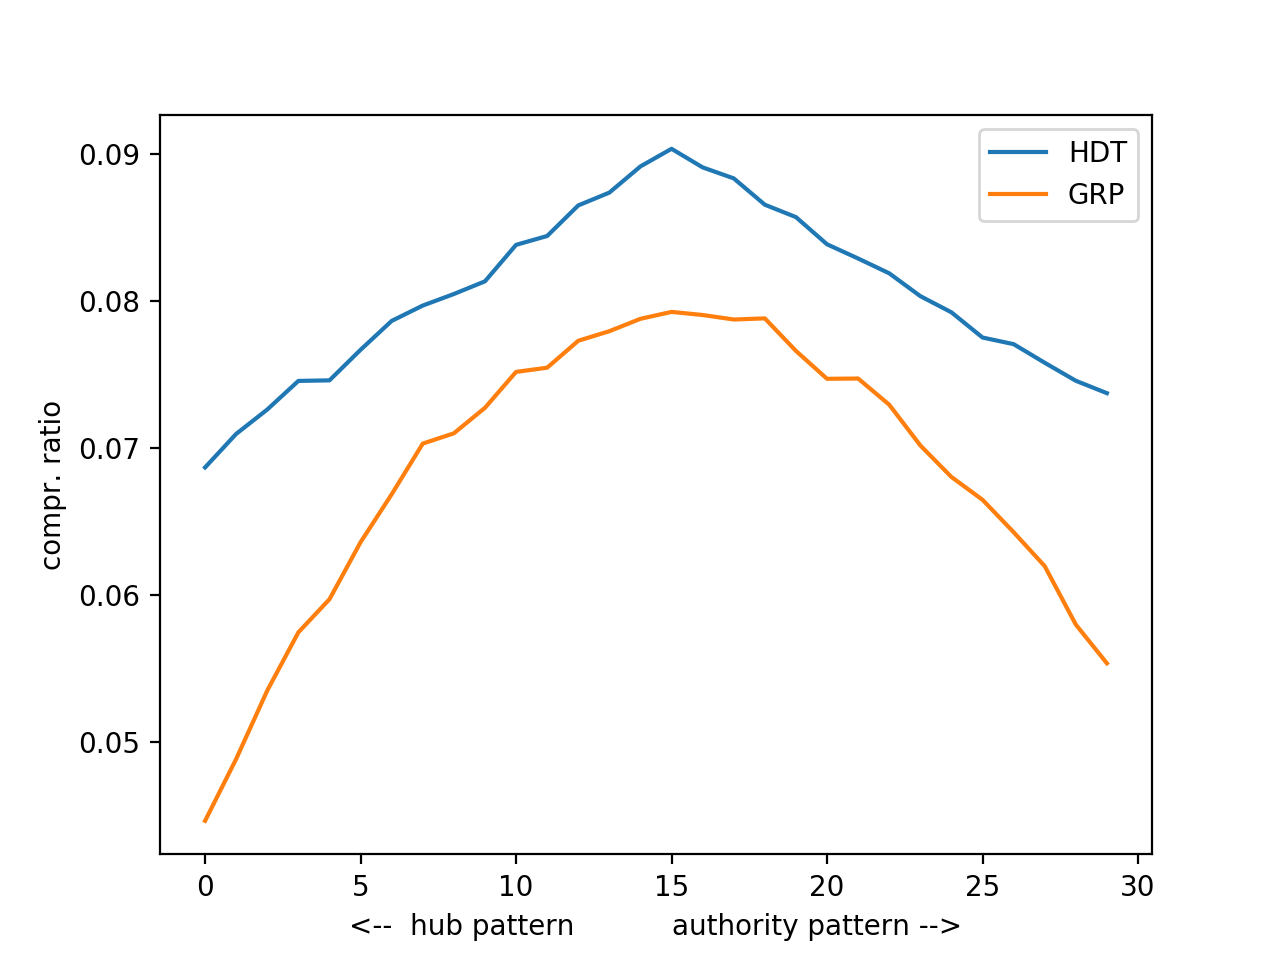
\includegraphics[width=0.5\textwidth]{figures/GRPvsHDT/bothWithDict}\label{fig:ratiosBothWithDict}}
	\caption{The compression ratios for GRP and HDT without and with dictionary sizes.}
\end{figure}

One could now argue that only one distinct predicate was used in that scenario and this is beneficial for GRP, as it gets worse as the number of predicates increases. Therefore a further evaluation is made in Fig.~\ref{fig:bothwithdict1000predicates}, where 1000 distinct predicates have been used. That is a quite high number considering the number of triples (1199) compared to real RDF data \todo{belegen}. One can see that the compression ratios are now higher for both compressors, but still GRP's ratio is always smaller than HDT's. HDT's ratio is still 1.7 times higher on average. So, the increasing number of predicates has a similar effect on both algorithms.

\begin{figure}
	\centering
	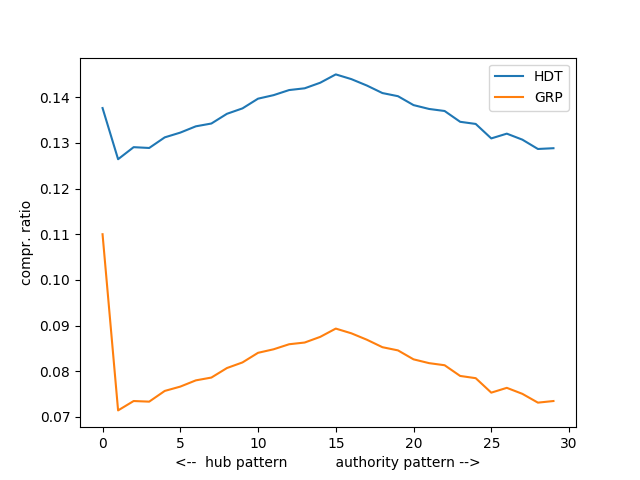
\includegraphics[width=0.7\linewidth]{figures/GRPvsHDT/bothWithDict1000Predicates}
	\caption{The compression ratios for GRP and HDT with dictionary sizes. Graphs have now 1000 distinct predicates.}
	\label{fig:bothwithdict1000predicates}
\end{figure}

Apart from the compression ratio, the run time is also important for the overall performance. Fig.~\ref{fig:runtimes} shows the average run times of the two algorithms. For this the same scenario with the star pattern (and only one distinct predicate) was used. It has been executed 100 times to get a sophisticated run time measurement, because the run time also depends on the current CPU workload of the computer.

\begin{figure}
	\centering
	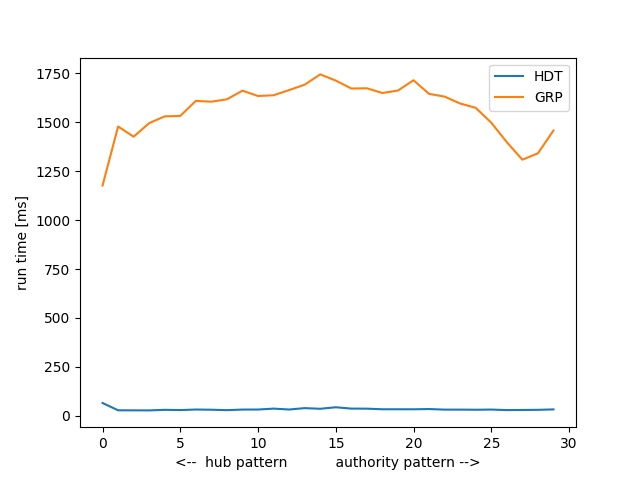
\includegraphics[width=0.7\linewidth]{figures/GRPvsHDT/runtimes}
	\caption{Run times of both algorithms (average run time of 100 consecutive executions).}
	\label{fig:runtimes}
\end{figure}


It can be seen that the runtime of GRP is significantly higher than that of GRP. It is on average ca. 48 times as high.

However, it should also be noted that the implementation of GRP is rather rudimentary  (according to the authors of~\cite{maneth}), while that of HDT has been under development for some time. So they are not comparable in terms of quality. Unfortunately, one cannot say at this point whether a more professional implementation of GRP will also be slower than HDT.

In addition one can notice that GRP's run time fluctuates more than that of HDT. GRP has a standard deviation of about 134, while HDT only has a standard deviation of about 7. One reason for this is that GRP, in contrast to HDT, is non-deterministic because of the partly random search order of the graph. On the other hand, the high deviations are also a confirmation of the above mentioned hypothesis that the behavior of GRP depends more on the structure of the input data than HDT does.



\section{Compression Ratio Improvements}

\subsection{Ontology Knowledge}\label{sec:evaluationOntKnowledge}

\subsection{Dictionary Improvements}\label{sec:evaluationDictImprovements}
















